\paragraph{Tuning the baseline.} The 0.8 threshold of the rule curve was an
arbitrary first choice. To give the agent a fair opponent, we also
grid-searched the threshold on 30 separate \emph{tuning} seeds
($20{,}000$--$20{,}029$; Figure~\ref{fig:tuning}). The best value, a flood
rule that starts releasing above 0.4\,$\Scap$, is then
evaluated on the same test seeds as everything else (``Tuned rule'').

\begin{figure}[h]
\centering
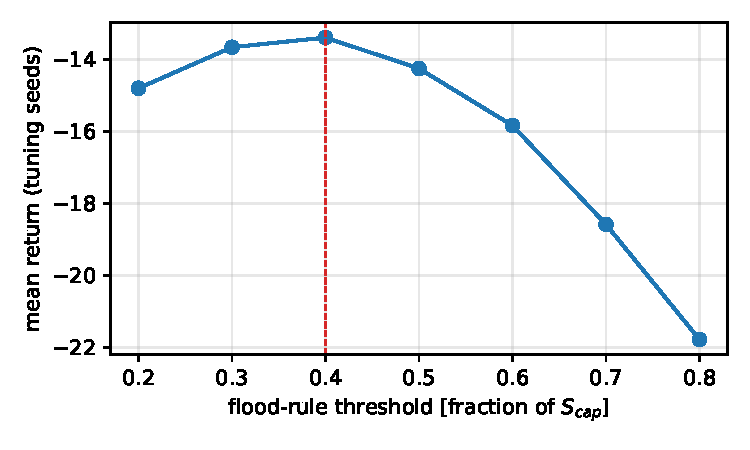
\includegraphics[width=0.5\textwidth]{figures/threshold_tuning.pdf}
\caption{Mean return of the rule curve versus its flood-rule threshold, on
the tuning seeds.}
\label{fig:tuning}
\end{figure}

\paragraph{Paired comparison.} Because every policy sees the same 30 storm
sequences, the fair test is the per-episode difference in return
(Table~\ref{tab:paired}). The spread in Table~\ref{tab:results} is
dominated by how stormy each season is, and this pairing cancels it.

\begin{table}[h]
\centering
\begin{tabular}{lrrr}
\toprule
baseline & mean(PPO $-$ baseline) & std.\ error & PPO better in \\
\midrule
Demand only & $+23.39$ & 4.01 & 23/30 \\
Rule curve (0.8) & $+7.54$ & 2.11 & 20/30 \\
Tuned rule (0.4) & $+0.79$ & 0.86 & 12/30 \\
\bottomrule
\end{tabular}

\caption{Paired differences in episode return, PPO minus baseline, on the
30 test episodes.}
\label{tab:paired}
\end{table}

\paragraph{What the agent learned.}
\begin{itemize}
\item PPO clearly beats releasing the demand only (by about 23 return
points) and the untuned rule curve (by about 7.5 points, better in 20 of 30
episodes). It cuts the flood penalty roughly in half and the spill penalty
by a factor of about two.
\item It does this with a \emph{drawdown hedging} strategy
(Figure~\ref{fig:traj_best}). PPO releases more than the demand most of the
time and keeps the reservoir low, so storms are absorbed instead of
spilled. The cost is a higher supply deficit (6\% versus 2\% of demand)
and occasional near-empty periods. The policy map
(Figure~\ref{fig:policymap}) shows the release increasing smoothly with
both storage and the forecast inflow.
\item Against the \emph{tuned} rule curve the difference is
$+0.8\pm0.9$, i.e.\ statistically indistinguishable. In effect, PPO
rediscovered ``keep the reservoir around 40\% full and release the
excess'', which is close to the best policy in the rule-curve family for
this reward. The two policies reach the same return differently: the tuned
rule floods on fewer days, while PPO exceeds $\Qsafe$ more often but by
smaller margins.
\end{itemize}

\paragraph{Interpretation.} For a single reservoir with a 3-day forecast
and this reward, a well-tuned one-parameter rule is already near-optimal.
RL earns its keep only when that stops being true, for example with
multiple interacting reservoirs, nonlinear water-quality objectives,
longer forecasts whose skill varies, or rewards that a fixed rule cannot
express. The value of this exercise is the pipeline: the same
environment-and-agent code applies unchanged to richer OHQ models.
